\notechapter{N-20221214}{Tarski's Circle-Squaring Problem: From Polygon Dissection to Borel Equidecomposition}

\section{The route of the note}

This note is about Tarski's circle-squaring problem, but the source pages do not treat it as a single isolated puzzle.  They move through a sequence of increasingly subtle notions:
\[
\begin{gathered}
  \text{Tarski circle-squaring}\longrightarrow \text{Hilbert's third problem}\\
  \longrightarrow \text{measure and paradoxical decomposition}\\
  \longrightarrow \text{Laczkovich's theorem}\longrightarrow \text{Borel circle squaring}.
\end{gathered}
\]
The figures below are kept only when the visual configuration itself matters.  The surrounding theorem statements, comments, formulas, and handwritten annotations have been incorporated into the prose.

Tarski asked in 1925 whether a disk and a square of equal area in the plane are equidecomposable: can the disk be partitioned into finitely many pieces, and can those pieces be moved by isometries to partition the square?

\section{Equidecomposability and dissection congruence}

Let a group $G$ act on a set $X$.  Two subsets $A,B\subseteq X$ are $G$-equidecomposable if there are finite partitions
\[
  A=A_1\sqcup\cdots\sqcup A_m,
  \qquad
  B=B_1\sqcup\cdots\sqcup B_m,
\]
and elements $g_i\in G$ such that
\[
  g_i(A_i)=B_i.
\]
For plane polygons, one usually lets $G$ be the group of Euclidean isometries.  In that setting the classical language is dissection congruence: cut one polygon into finitely many polygonal pieces and rearrange them to obtain the other.

The first example is the familiar parallelogram-to-rectangle cut.

\begin{figure}[H]
\centering
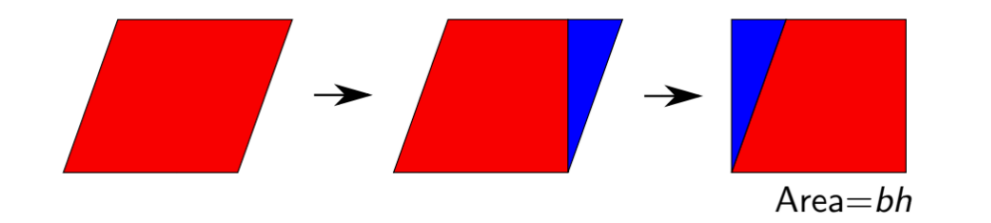
\includegraphics[width=.66\linewidth]{figures/N-20221214/01-parallelogram-to-rectangle.png}
\caption{A parallelogram dissected and rearranged into a rectangle.}
\end{figure}

Area is obviously preserved by dissection congruence.  The Wallace--Bolyai--Gerwien theorem says that, for plane polygons, area is also sufficient.

\begin{theorem}[Wallace--Bolyai--Gerwien]
Any two plane polygons of the same area are dissection congruent.
\end{theorem}

One small point in the note is transitivity.  If polygon $P$ is dissection congruent to $Q$, and $Q$ is dissection congruent to $R$, then $P$ is dissection congruent to $R$.  One refines the two dissections so that the intermediate polygon $Q$ is cut compatibly, then composes the rearrangements.

\begin{figure}[H]
\centering
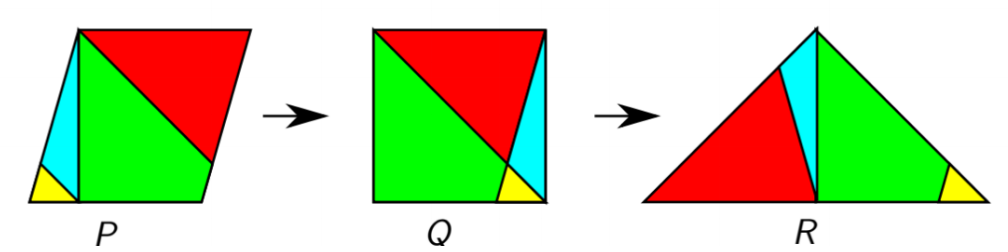
\includegraphics[width=.72\linewidth]{figures/N-20221214/02-polygon-transitivity-PQR.png}
\caption{The transitivity intuition: a dissection from $P$ to $Q$ and one from $Q$ to $R$ compose.}
\end{figure}

The proof of the theorem is constructive.  First chop a polygon into triangles.

\begin{figure}[H]
\centering
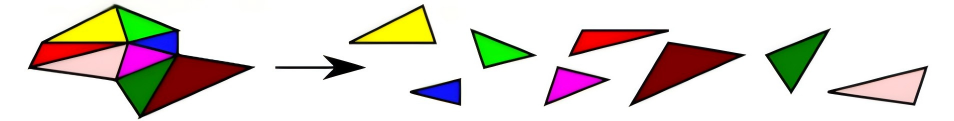
\includegraphics[width=.76\linewidth]{figures/N-20221214/03-polygon-triangulation.png}
\caption{The first reduction: chop a polygon into triangles.}
\end{figure}

Then dissect each triangle into a parallelogram and then a rectangle; dissect each rectangle into a square; combine squares by the Pythagorean dissection.

\begin{figure}[H]
\centering
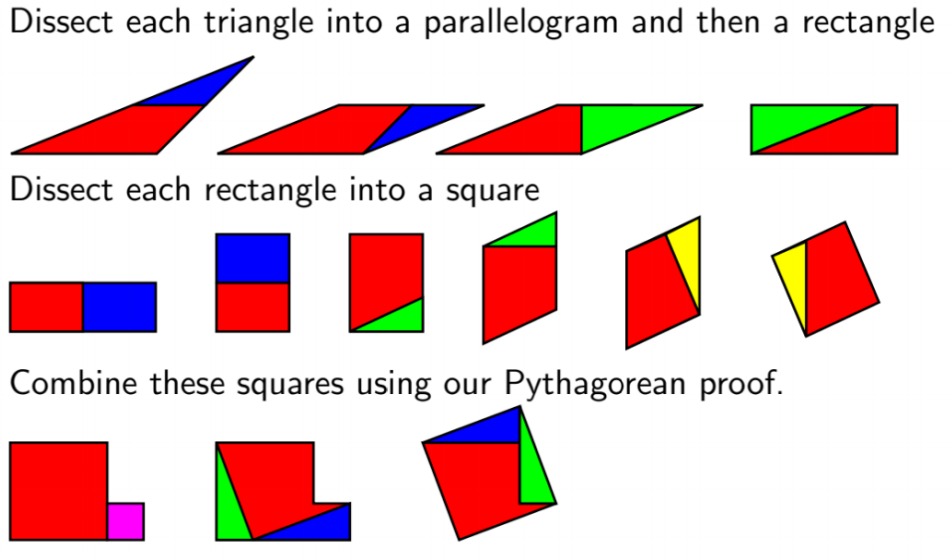
\includegraphics[width=.75\linewidth]{figures/N-20221214/04-triangle-rectangle-square-chain.png}
\caption{The visual chain: triangle to parallelogram/rectangle, rectangles to squares, then combine squares.}
\end{figure}

The theorem establishes the baseline: for tame plane polygons, equal area exactly characterizes finite dissection congruence.

\section{Hilbert's third problem and the Dehn invariant}

Hilbert's third problem asks whether equal volume similarly characterizes dissection congruence of three-dimensional polytopes.  Dehn's theorem says no: a cube and a regular tetrahedron of the same volume are not dissection congruent.

The extra obstruction is the Dehn invariant.  If a polyhedron has edge lengths $\ell_i$ and corresponding dihedral angles $\theta_i$, the invariant has the form
\[
  D(P)=\sum_i \ell_i\otimes \theta_i
\]
with values in a tensor product such as $\mathbb R\otimes_{\mathbb Z} \mathbb R/(2\pi\mathbb Z)$, depending on conventions.  The invariant records length-angle data that volume does not see.  The handwritten note correctly marks the tensor product as a point worth noticing: this is not elementary area bookkeeping anymore.

Sydler's theorem says that volume and Dehn invariant together are complete in dimension three.  Thus the two-dimensional polygon theorem has no naive three-dimensional analogue.

\section{Measure-theoretic background}

The source page then discusses measure.  Vitali sets imply that for every $n\ge1$, there is no extension of Lebesgue measure to all subsets of $\mathbb R^n$ that is both countably additive and invariant under isometries.

If countable additivity is weakened to finite additivity, the dimension matters.  For $n\ge3$, the Banach--Tarski paradox shows that there is no such finitely additive isometry-invariant measure on all bounded sets compatible with volume.  For $n\le2$, Banach measures exist.  The note emphasizes the reason: in dimension at least three, the isometry group contains enough free-group behavior to allow paradoxical decompositions; in dimensions one and two it does not.

For Tarski's problem in the plane, this means that equal area is still a necessary condition.  A disk and square that are equidecomposable by isometries must have the same Lebesgue measure, even if the pieces themselves are nonmeasurable.

\section{Tarski's circle-squaring problem}

The central question is then:

\begin{quote}
Are a disk and a square in $\mathbb R^2$ of the same area equidecomposable?
\end{quote}

\begin{figure}[H]
\centering
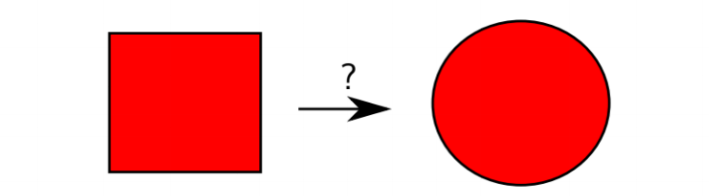
\includegraphics[width=.55\linewidth]{figures/N-20221214/05-disc-square-question.png}
\caption{The central visual question: equal-area disk and square.}
\end{figure}

At first sight the boundary seems to obstruct the construction.  A disk has circular boundary; a square has straight boundary.  This intuition is correct for a stricter notion, but not for arbitrary equidecomposition.

\section{Scissors congruence and why nice pieces fail}

The note distinguishes equidecomposability from scissors congruence.  In the scissors-congruence version, the pieces must be tame: each piece is homeomorphic to a disk and has boundary given by curves of finite length.  Under such restrictions, the disk and square are not scissors congruent.

The invariant mentioned in the source is:
\[
  \text{convex circular perimeter}-\text{concave circular perimeter}.
\]
When a curved circular arc is created inside a dissection, it is paired with an opposite concave arc, so the internal contributions cancel.  The remaining outer boundary contribution is preserved.  A disk has a nonzero circular-boundary contribution, while a square has none.  Hence a disk and square cannot be scissors congruent in this tame sense.

\begin{figure}[H]
\centering
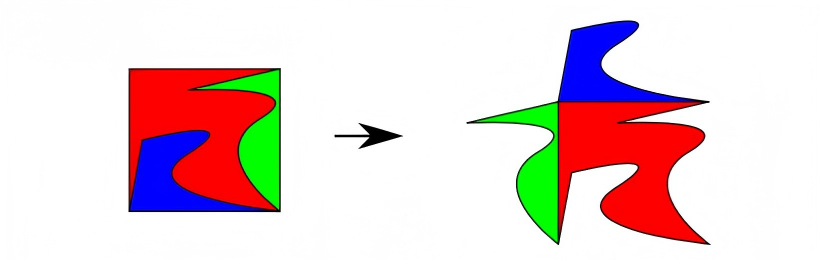
\includegraphics[width=.58\linewidth]{figures/N-20221214/06-scissors-congruence-pieces.png}
\caption{Tame scissors pieces preserve circular-boundary information.}
\end{figure}

This is the first major subtlety: the positive answer to Tarski's problem requires pieces much wilder than ordinary scissors pieces.

\section{Laczkovich's positive theorem}

Laczkovich proved in 1990 that Tarski's circle-squaring problem has a positive answer.  In 1992 he proved a broader theorem.  A simplified statement is:

\begin{theorem}[Laczkovich]
Let $A,B\subseteq \mathbb R^k$ be bounded sets with the same positive Lebesgue measure.  If the boundaries of $A$ and $B$ have upper Minkowski dimension strictly less than $k$, then $A$ and $B$ are equidecomposable by translations.
\end{theorem}

For a disk and square in the plane, the boundaries are one-dimensional, so the hypothesis applies.

The proof does not draw a literal jigsaw.  It converts the problem into a bounded matching problem in a graph generated by translations.

\section{First idea: work in the torus}

Scale and translate $A$ and $B$ so that they lie inside $[0,1)^k$.  Identify this cube with the $k$-torus
\[
  \mathbb T^k=(\mathbb R/\mathbb Z)^k.
\]
Then $A$ and $B$ are equidecomposable by translations as subsets of the torus iff, after possibly using more pieces, they are equidecomposable by translations in $\mathbb R^k$.

\begin{figure}[H]
\centering
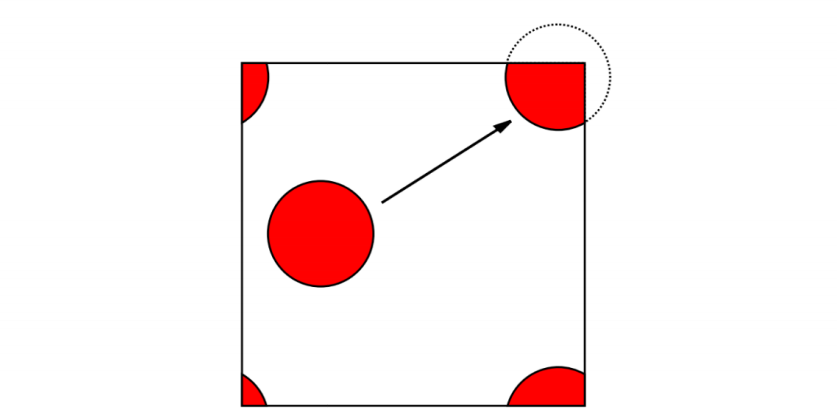
\includegraphics[width=.48\linewidth]{figures/N-20221214/07-torus-wraparound.png}
\caption{Working on the torus: translations wrap around the fundamental cube.}
\end{figure}

This torus reduction matters because translations become an action on a compact group.  Compactness and periodic boundary conditions make the orbit structure manageable.

\section{Random translations and a free action}

Choose a sufficiently large integer $d$ and random translations
\[
  u_1,\ldots,u_d\in\mathbb T^k.
\]
They define an action of $\mathbb Z^d$ on $\mathbb T^k$ by
\[
  (n_1,\ldots,n_d)\cdot x
  =n_1u_1+\cdots+n_du_d+x.
\]
For almost every choice of the $u_i$, this action is free: no nonzero element of $\mathbb Z^d$ fixes a point.  Thus each orbit can be visualized as a copy of $\mathbb Z^d$.

\begin{figure}[H]
\centering
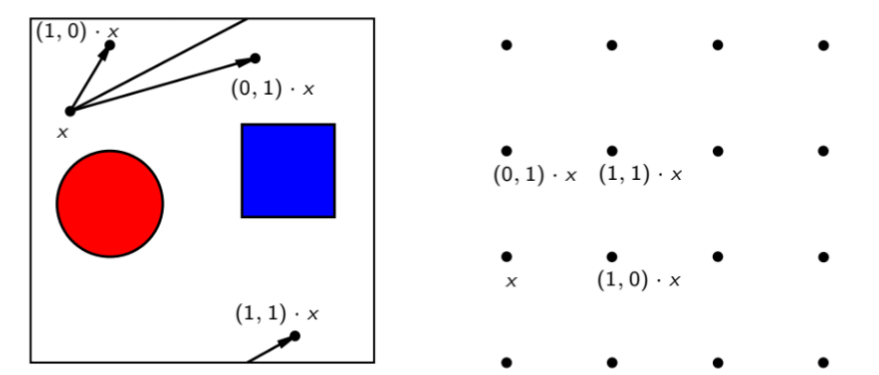
\includegraphics[width=.68\linewidth]{figures/N-20221214/08-random-translations.png}
\caption{Random translations generate lattice-like orbits on the torus.}
\end{figure}

\section{The graph and bounded-distance bijection}

Define a graph $G$ with vertex set $\mathbb T^k$.  Two points $x,y$ are adjacent if there exists $g\in\mathbb Z^d$ with
\[
  g\cdot x=y,
  \qquad
  \|g\|_\infty=1.
\]
So edges correspond to single generator moves.

\begin{figure}[H]
\centering
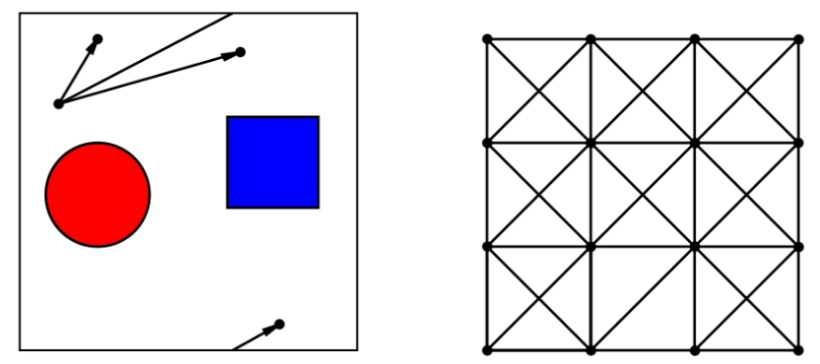
\includegraphics[width=.64\linewidth]{figures/N-20221214/09-graph-generator-grid.png}
\caption{The generator graph: locally it looks like a lattice with bounded moves.}
\end{figure}

To show $A$ and $B$ are equidecomposable, it suffices to find a Borel bijection
\[
  f:A\to B
\]
of bounded distance in $G$: there is some fixed $N$ such that
\[
  d_G(x,f(x))\le N
  \qquad \text{for all }x\in A.
\]
If such an $f$ exists, then only finitely many group elements $g$ can occur.  Put
\[
  A_g=\{x\in A:f(x)=g\cdot x\}.
\]
The sets $A_g$ partition $A$, and the translated sets $g\cdot A_g$ partition $B$.  This gives the desired finite equidecomposition.

This is the conceptual heart of the proof:
\[
  \text{finite translation equidecomposition}
  \quad\Longleftarrow\quad
  \text{bounded-distance orbit matching}.
\]

\section{Orbit matching}

Inside a single orbit of the $\mathbb Z^d$ action, the problem becomes matching red $A$-points to blue $B$-points by bounded paths.

\begin{figure}[H]
\centering
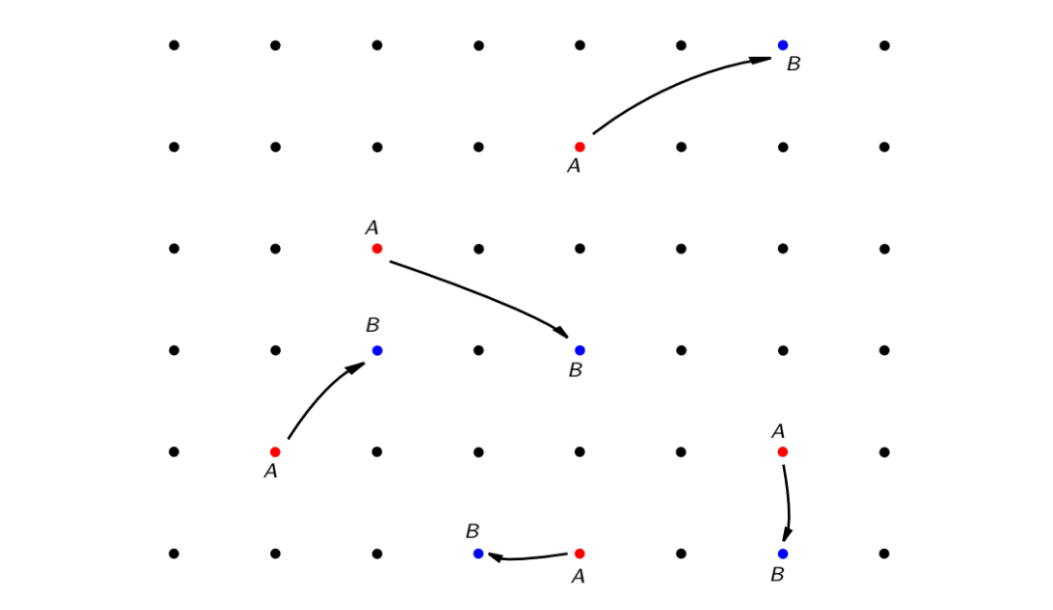
\includegraphics[width=.66\linewidth]{figures/N-20221214/10-orbit-matching.png}
\caption{Within one orbit, equidecomposition becomes a matching problem.}
\end{figure}

A bounded matching can exist only if large finite regions of the orbit contain approximately the same number of $A$-points and $B$-points.  This leads to discrepancy estimates.

\section{Discrepancy estimates}

For an orbit point $x$, define a finite box
\[
  S_N(x)=\{(n_1,\ldots,n_d)\cdot x:0\le n_i<N\}.
\]
Ergodic intuition suggests
\[
  |S_N(x)\cap A|\approx \lambda(A)N^d.
\]
The handwritten note warns that this is only a heuristic: ordinary ergodic theorems alone are not strong enough.  Laczkovich needs a uniform quantitative estimate from Diophantine approximation and discrepancy theory.

\begin{figure}[H]
\centering
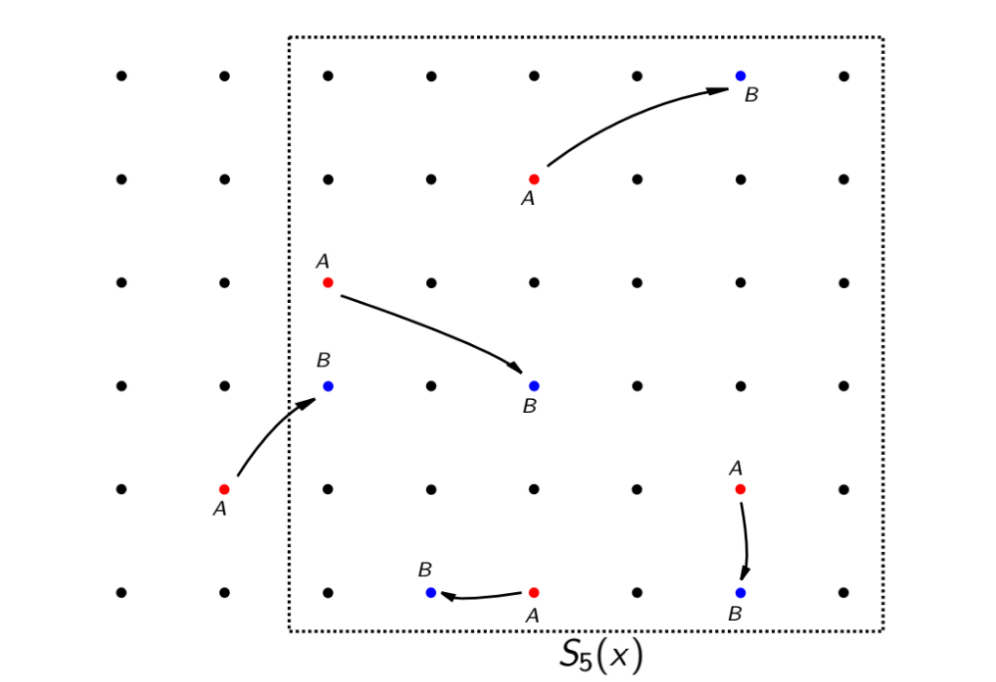
\includegraphics[width=.62\linewidth]{figures/N-20221214/11-discrepancy-box.png}
\caption{A finite orbit box $S_N(x)$; discrepancy compares observed counts with expected measure.}
\end{figure}

The key lemma states that there exist $\varepsilon>0$ and $M$ such that for all $x$ and $N$,
\[
  \left||S_N(x)\cap A|-\lambda(A)N^d\right|
  \le MN^{d-1-\varepsilon},
\]
and similarly for $B$:
\[
  \left||S_N(x)\cap B|-\lambda(B)N^d\right|
  \le MN^{d-1-\varepsilon}.
\]
Since $\lambda(A)=\lambda(B)$, large boxes contain nearly equal numbers of $A$ and $B$ points.  The error term grows more slowly than the volume term $N^d$, which is exactly what makes matching possible.

\section{From Laczkovich to Borel circle squaring}

Laczkovich's original proof used the axiom of choice.  Later work by Marks and Unger showed that the pieces can be chosen Borel.  This is much stronger: the pieces are still extremely complicated, but they are definable in the Borel hierarchy.

\begin{figure}[H]
\centering
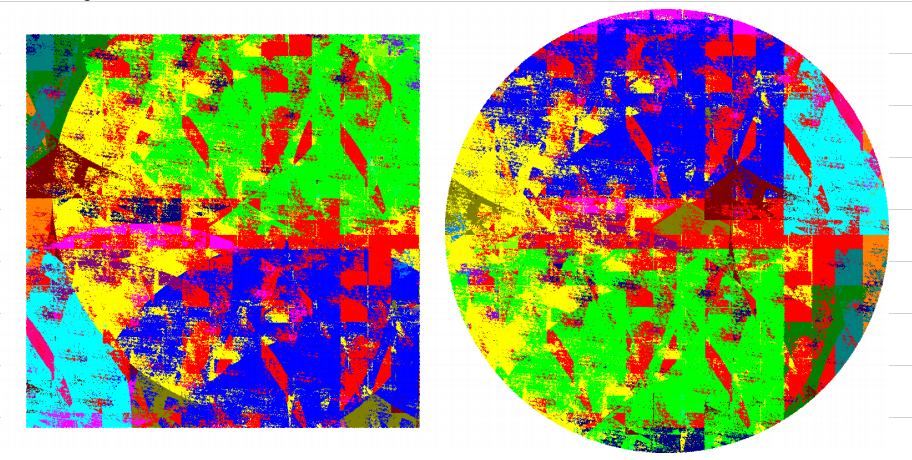
\includegraphics[width=.60\linewidth]{figures/N-20221214/12-borel-colored-partition.png}
\caption{A visual impression of the Borel circle-squaring pieces.}
\end{figure}

The final handwritten note says the main components are: Dehn invariant, group action, torus embedding, traversal/matching, and measure/discrepancy theory.  That summary is accurate.  The proof is not one trick; it is a combination of several fields.

\section{Expanded synthesis and advanced context}

The same question changes answer depending on the category of pieces.  Plane polygons are controlled by area.  Three-dimensional polyhedra require the Dehn invariant.  Tame planar scissors pieces preserve circular-boundary data, so a disk cannot become a square.  But arbitrary or Borel pieces are flexible enough for Laczkovich's theorem and Borel circle squaring.

Thus Tarski's circle-squaring problem is a crossroads of geometry, measure theory, group actions, discrepancy estimates, graph matching, and descriptive set theory.  The important lesson is not only that the answer is yes, but why the yes lives far beyond ordinary scissors geometry.


\paragraph{Expanded synthesis.}
The elementary geometric content of this chapter should be read through transformations and invariants. The earlier sections (`The route of the note`, `Equidecomposability and dissection congruence`, `Hilbert's third problem and the Dehn invariant`, `Measure-theoretic background`, `Tarski's circle-squaring problem`) may use coordinates, angles, determinants, parametrizations, or integral formulas, but the organizing question is: which quantities survive the transformations naturally associated with the problem? Euclidean geometry preserves distances and angles; affine geometry preserves lines and ratios on a line; projective geometry preserves incidence and cross ratio; differential geometry preserves coordinate-independent objects such as forms, metrics, and orientations.

This perspective separates different layers of a problem. A dot product belongs to metric geometry. A determinant belongs to oriented volume. A cross ratio belongs to projective geometry. A line or surface integral of a differential form belongs to oriented topology. A scalar area integral belongs to the metric-induced measure. Confusing these layers is the source of many errors, especially in vector calculus where $dS$, $F\cdot n\,dS$, $dx\wedge dy$, and boundary orientation look similar but encode different structures.

When returning to the original examples, identify the natural object before computing. If the problem is about concurrence or collinearity, projective or affine tools may be natural. If it is about distance, angle, or orthogonality, metric tools are essential. If it is about flux or circulation, differential forms and orientation explain the signs. The advanced viewpoint makes the elementary solution more disciplined rather than more abstract for its own sake.
